\section{Klassische Enterprise-Architektur}

%%%%%%%%%%%%%%%%%%%%%%%%%% Monolithic Architecture %%%%%%%%%%%%%%%%%%%%%%%%%%%

\begin{frame}{Monolithic Architecture}
    \begin{itemize}
        \item Monolith ist altgriechisch für \textit{einheitlicher Stein}
        \item Einheitlich: Alles ist eins - alle Funktionalitäten in einer Komponente
        \item Stein: Altes Material - früher gut. Heute schlecht?
        \item Problem: Enge Kopplung
    \end{itemize}
\end{frame}

\begin{frame}{Monolithic Architecture: Beispiel E-Commerce}
    \begin{figure}[!h]
        \centering
        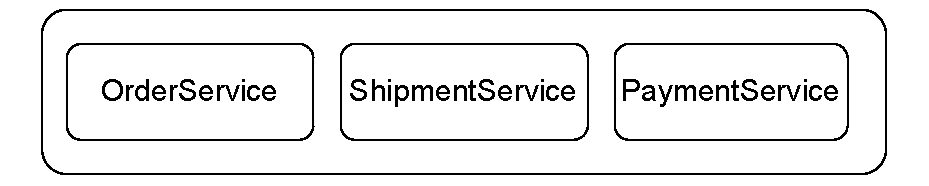
\includegraphics[scale=0.70]{imglib/mono/mono}
        \caption{E-Commerce-Beispiel mit Monolithic Architecture}
        \label{fig:mono-ecommerce}
    \end{figure}
\end{frame}

\begin{frame}{Monotlithic Architecture: Agilität}
    \begin{itemize}
        \item Enge Kopplung ist fatal
        \begin{itemize}
            \item Keine kleinen autonomen Teams
            \item Erhöhte Komplexität und schwere Wartung $\Rightarrow$ längere Iterationen $\Rightarrow$ unflexibel
            \item Funktionalitäten nicht wiederverwendbar $\Rightarrow$ Mehraufwand \& Duplikation $\Rightarrow$ Änderungen teuer
            \item Isolierte Funktionstests sind möglicherweise aufwendig
        \end{itemize}
        \item Auslieferung nur im Ganzen \& längere Iterationen $\Rightarrow$ seltene Auslieferung
        \item Verpflichtung auf genau eine Technologie
        \item Horizontale Skalierung kaum möglich
        \item Aber: System ist nicht verteilt $\Rightarrow$ Keine Intersystemkommunikation $\Rightarrow$ Geringe Time-to-Market \& möglicherweise einfache System-Tests
    \end{itemize}
\end{frame}

%%%%%%%%%%%%%%%%%%%%%%%%%% Modular Monolithic Architecture %%%%%%%%%%%%%%%%%%%%%%%%%%%

\begin{frame}{Modular Monolithic Architecture}
    \begin{itemize}
       \item Bisher: Eine eng gekoppelte Komponente
       \item Jetzt: Eine Komponente mit lose gekoppelten Teil-Funktionalitäten (Modulen)
       \item Evolution monolithischer Architektur, um Komplexität zu verringern
     \end{itemize}
\end{frame}

\begin{frame}{Monolith Architecture: Beispiel E-Commerce II}
    \begin{figure}[!h]
        \centering
        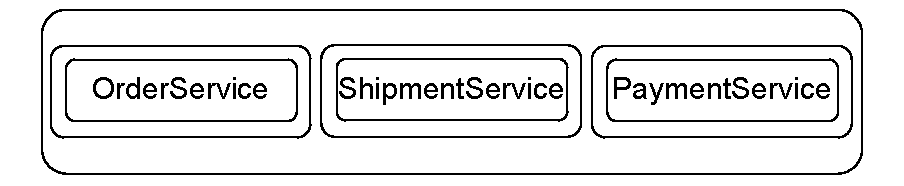
\includegraphics[scale=0.70]{imglib/mono/mono-example}
        \caption{E-Commerce-Beispiel mit Modular Monolithic Architecture}
        \label{fig:mono-modular}
    \end{figure}
\end{frame}

\begin{frame}{Modular Monolithic Architecture: Agilität}
    \begin{itemize}
        \item Im Vergleich zu Monolith: Verbesserungen bezüglich Entwicklung
        \begin{itemize}
            \item Reduzierte Komplexität $\Rightarrow$ bessere Wartbarkeit
            \item Modularisierung ermöglicht kleine semi-autonome Teams
        \end{itemize}
        \item Noch immer problematisch:
        \begin{itemize}
            \item Deployment im Ganzen
            \item Keine horizontale Skalierung
            \item Keine Wiederverwendbarkeit von Funktionalitäten
        \end{itemize}
    \end{itemize}
\end{frame}

%%%%%%%%%%%%%%%%%%%%%%%%%% Service-oriented Architecture %%%%%%%%%%%%%%%%%%%%%%%%%%

\begin{frame}{Service-oriented Architecture}
    \begin{itemize}
        \item Bisher: Eng gekoppelte Funktionalitäten
        \item Jetzt: Lose Kopplung von Funktionalitäten durch Kapselung als Dienst
        \item Ziel Service-oriented Architecture (SOA): Wiederwendung von Funktionalitäten
    \end{itemize}
\end{frame}

\begin{frame}{Service-oriented Architecture: Komponenten}
    \begin{itemize}
        \item Service Provider: Stellt spezifischen Dienst bereit
        \item Service Consumer: Nutzt bereitgestellten Dienst
        \item Broker: Vermittler, der Kommunikation zwischen Consumer und Provider regelt
        \item Service Registry: Sammlung von Metadaten zu Services und deren Provider
    \end{itemize}
\end{frame}

\begin{frame}{Service-oriented Architecture: Struktur}
    \begin{figure}[!h]
        \centering
        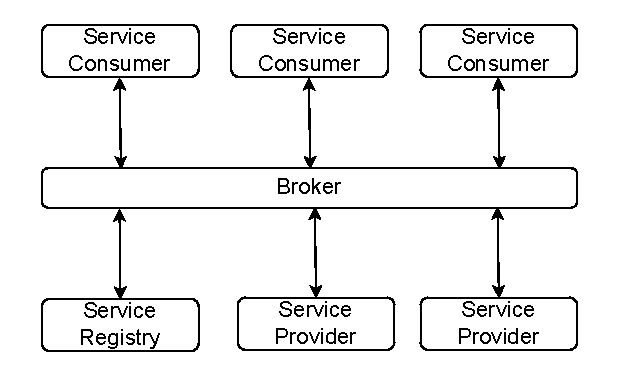
\includegraphics[scale=0.80]{imglib/soa/soa}
        \caption{Aufbau der Service-oriented Architecture}
        \label{fig:soa}
    \end{figure}
\end{frame}

\begin{frame}{Service-oriented Architecture: Beispiel E-Commerce I}
    \begin{itemize}
        \item \texttt{OrderService}: Dienst für Verwaltung von Bestellungen
        \item \texttt{PaymentService}: Dienst für die Abwicklung von Zahlungen (Service von PayPal, \ldots)
        \item \texttt{ShipmentService}: Dienst für den Versand (Service von DHL, \ldots)
    \end{itemize}
\end{frame}

\begin{frame}{Service-oriented Architecture: Beispiel E-Commerce II}
    \begin{figure}[!h]
        \centering
        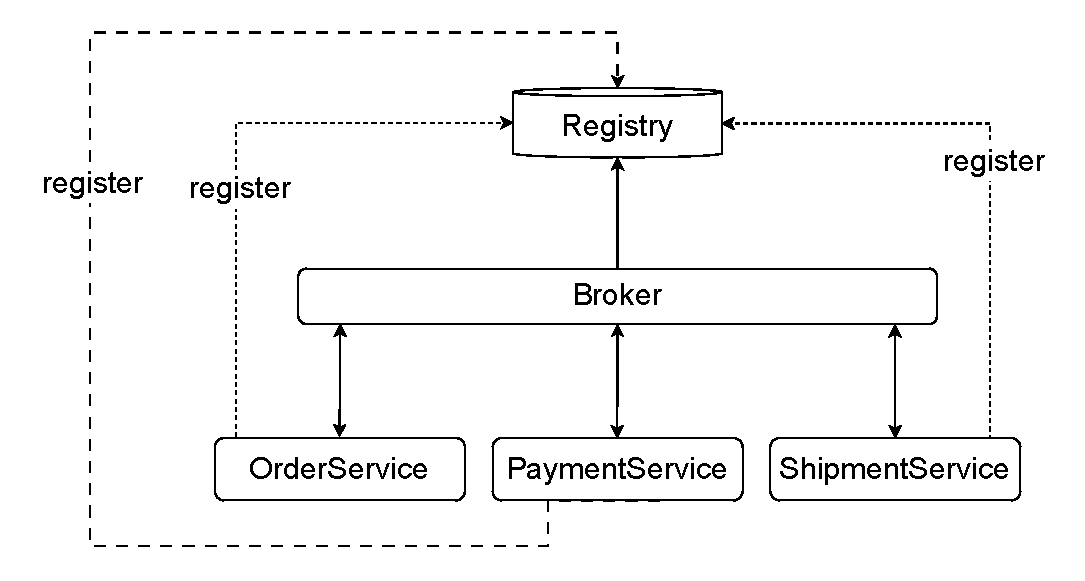
\includegraphics[scale=0.50]{imglib/soa/soa-example}
        \caption{E-Commerce-Beispiel mit Service-oriented Architecture}
        \label{fig:soaecommerce}
    \end{figure}
\end{frame}

\begin{frame}{Service-oriented Architecture: Agilität}
    \begin{itemize}
        \item Wie bei modularem Monolithen: Lose Kopplung $\Rightarrow$ kleine autonome Teams
        \item Aber zusätzlich: Deployment in Teams $\Rightarrow$ kürzere Iterationen \& häufigere Auslieferung
        \item Dadurch: Flexibler gegenüber wechselnden Anforderungen
        \item Zeit- und Kosteneinsparungen durch Wiederverwendung von Diensten
        \item Aber: Langfristig Abhängigkeiten zwischen Diensten, besonders für grob-granulare Dienste
    \end{itemize}
\end{frame}